%\documentclass{article}
%\input{C:/D/Research/my_latex_defs.tex}
%\begin{document}

The methods section proceeds as follows.  First, we explain the experimental paradigm under consideration. Next, we describe the model used to solve the two problems of interest.  Because the mathematical tools used to solve these problems may be unfamiliar, a brief tutorial is then provided.  Finally, we apply these tools to the model at hand.

\subsection{Experimental Paradigm} \label{sec:exp}

We are interested in providing useful computational tools for the following experimental paradigm.  Calcium sensitive fluorophores are in some neurons  of interest, and (mostly) not elsewhere.  When these neurons spike, the intracellular concentration of calcium in the soma jumps up and then decays back down to rest. The magnitude of the fluorescence signal is approximately proportional to the calcium concentration.  An image acquisition system collects the fluorescent signal at some rate. The spiking activity of these neurons may be partially governed by some external sensorimotor covariates, such as pictures, sounds, or body movements.

Two problems are ubiquitous given this experimental paradigm.  First, when did the observable neurons spike?  The answer to this question is difficult to obtain for a number of reasons, including that the data collection is both (i) noisy, in that the fluorescence signals may not perfectly coincide with the actual calcium fluctuations, and (ii) intermittent, in that the frame rate may be slower than the dynamics of interest.  Second, what causes the neurons to spike?  The causes we consider include spontaneous activity, the external environment, and intrinsic dynamics of the neurons.  Below, we develop a model based on this experimental paradigm, designed specifically to answer these two questions.

\subsection{Model} \label{sec:model}

To model this scenario, we first discretize the experimental time course, into $T$ time steps of size $dt$, indexed by $t$, i.e., $t \in [0,T] = \mathcal{T}$,\footnote{Throughout this text, we use the standard notation that $(x_0,x_n]$ refers to the sequence of all $x_i$ where $i$ is between 1 and n (i.e., excluding $i=0$ but including $i=n$).} where $\mathcal{T}$ is the set of all time steps.  We then assume that at each time step, the neuron has some probability, $p_t$, of emitting a spike, which is a function of the input to the neuron at that time, $y_t$.  One can therefore write the probability governing the spiking of the neuron as a Bernoulli distribution, conditioned on the input

\begin{equation} \label{eq:p_t}
\begin{split}
p_t &= \p[n_t =1 | y_t] = 1 - e^{-f(y_t) dt}\\
1-p_t&=\p[n_t=0|y_t] =e^{-f(y_t) dt}
\end{split}
\end{equation}

\noindent where $n_t$ is the number of spikes emitted by the neuron at time $t$ (constrained to be zero or one here), $f(\cdot)$ is some potentially nonlinear function, and $\ve{\theta}$ is the vector of parameters governing the model (to be explained below).  This particular neural model has several desirable properties.  First, the $dt$ ensures that the neuron firing rate is independent of the discretization.  Second, as the magnitude of the input increases, so does the probability of firing.  Third, the likelihood of this function has no non-global extrema, so that one can quickly estimate the parameters of the model using any gradient ascent technique\cite{EscolaPaninski07}.  For this third property to hold, $f(\cdot)$ must be both convex and log-concave (a typical example is $f(\cdot)= \exp\{\cdot\}$).

We then assume that the input to the neuron is a sum of three terms: (i) a bias term setting the baseline firing rate, (ii) the linearly filtered stimulus, and (iii) spike histories:

\begin{align} \label{eq:y_t}
y_t = b + \ve{k}' \ve{x}_t + \ve{\omega}' \ve{h_t}
\end{align}

\noindent where $b$ is the bias term, $\ve{k}$ is the $D$-dimensional linear filter, $\ve{x}_t$ is the $D$-dimensional time-varying stimulus, and $\ve{h}_t=(h_{lt})_{l=1}^L$ and $\ve{\omega}=(\omega_l)_1^L$ are the $L$ spike history terms and their associated weights. The spike history terms are included to enable the model to account for complex refractory effects, such as bustiness or adaptation\cite{Paninski04}. For the spike history terms to fit within the SMC-EM framework developed below, they should adhere to two constraints: (i) they should comprise a convenient basis set, such that they can model arbitrary dynamics with relatively few parameters, and (ii) they should be Markovian.  These two constraints may be fulfilled by letting each spike history term be an exponential function with a unique time constant:

\begin{align} \label{eq:h_t}
h_{lt} - h_{l,t-1} = \frac{dt}{\tau_c} h_{l,t-1}  + n_{t-1} + \varepsilon_{lt}%, \qquad \varepsilon_{mt} \sim \mathcal{N}[\varepsilon_{mt}; 0,\sigma_{h_m}^2 dt]
\end{align}

\noindent where $h_{lt}$ is the value of spike history term $l$ at time $t$, and $\tau_{h_l}$ is its time constant.  $\varepsilon_{ht}$ is an additive Gaussian noise term with zero mean and variance $\sigma_{h_l}^2 dt$ (the $dt$ ensures that the variance is independent of the step size).  The activity of the observable neurons is measured using their intracellular calcium concentrations.  Experimental evidence suggests that after each action potential, the calcium concentration in the soma jumps, and subsequently decays back down to rest\cite{SmettersYuste99}.  Therefore, we model the calcium concentration, $C_t$ as:

\begin{align} \label{eq:C_t}
C_t - C_{t-1} = \frac{dt}{\tau_c} C_{t-1}   + \beta n_t + \varepsilon_{ct}%, \qquad \varepsilon_{ct} \sim \mathcal{N}[\varepsilon_{ct} ; 0,\sigma_c^2  dt]
\end{align}

\noindent where $\tau_c$ is the time constant, $\beta$ indicates the size of the jump. The noise term, $\varepsilon_{ct}$, accounts for the subthreshold calcium fluctuations, and is Gaussian with zero mean and $\sigma_c^2 dt$ variance.  We make two assumptions about the dynamics of the calcium sensors.  First, they fluoresce proportional to the concentration of calcium.  Second, their kinetics are fast enough relative to the calcium kinetics that they can be ignored.  Given those assumptions, the observations are simply

\begin{align} \label{eq:F_t}
F_t &= \alpha C_t + \gamma + \varepsilon_{Ft}%, \qquad \varepsilon_{Ft} \sim \mathcal{N}[\varepsilon_{Ft}; 0,\sigma_F^2  dt],
\qquad t \in\mathcal{T}_o
\end{align}

\noindent where $F_t$ is the fluorescence at time step $t$, $\alpha$ and $\gamma$ are the scale and shift term, respectively.  The noise term, $\varepsilon_{Ft}$, is Gaussian with zero mean and variance $\sigma_F^2  dt$. Note that (i) observations are noisy, and (ii) arrive only at a subset of times, $t \in\mathcal{T}_o \subseteq \mathcal{T}$, due to the slow frame rate, $f$.

Equations \eqref{eq:p_t}-\eqref{eq:F_t} can collectively be considered a cascade model, as depicted in Figure \ref{fig:mod}\textbf{(A)}. The cascade begins with the stimulus, $\ve{x}_t$, which is fed directly into the linear filter, $\ve{k}_t$.  The filtered stimulus is summed with the spike history terms from the previous time step, yielding the current input to the neuron, $y_t$.  This input is passed through the static nonlinearity, $1-e^{f(y_t) dt}$, providing the probability of spiking, $p_t$.  If the neuron spikes, $n_t=1$, both the spike history terms, $\ve{h}_t$ and the calcium concentration, $C_t$, jump.  Finally, some digital imaging device collects the fluorescence of the calcium sensors, $F_t$, from which one can construct the images used for analysis.

\begin{figure}
\centering
\includegraphics[width=1.0\linewidth]{neur_figs2}
\caption[Models]{Models.  \textbf{(A)} Cascade Model. The time-varying stimulus is first linearly filtered.  Then, the output of the filter passes through the nonlinearity.  The neuron subsequently spikes with probability.  If the neuron spikes, the intracellular calcium concentration jumps and then decays, as do the the spike history terms. Finally, an image is constructed from the resulting calcium sensitive fluorescence signal.  \textbf{(B)} Directed Acyclic Graphical Model. The horizontal dotted line divides the graph between the observed states (above the line) and hidden states (below the line). The graph depicts the conditional dependencies of the model by drawing directed edges (arrows) between the nodes (circles). The time step is indicated on the bottom.  The observations, $F_t$, are made intermittently. The hidden states (gray ellipses) are the calcium concentration, $C_t$, the spike trains, $n_t$, and the spike history terms, $\ve{h}_t$. Collective, they comprise a  Markov process.}
\label{fig:mod}
\end{figure}

\subsection{Computational Tools}

As mentioned earlier, given the aforementioned experimental paradigm, we are interested in solving two ubiquitous problems. First, we would like to find the underlying spike train from these noisy and intermittent observations, a type of problem typically referred to as \emph{inference}.  Second, we would like to fit the parameters of the model to the observations, a problem called \emph{learning}.  To solve these problems, we develop a Sequential-Monte-Carlo Expectation-Maximization (SMC-EM) algorithms. Because only a few neuroscientific investigations have used these methods\cite{GaoDonoghue02, BrockwellKass04, KellyLee04, SamejimaKimura04, HuysPaninski06b, Sanger07, ErgunBrown07}, this section provides a brief tutorial introducing these ideas in several steps.  First, we describe the problem in terms of a \emph{discrete-time state-space model} (DT-SSM).  Once in this formalism, we show how an \emph{Expectation-Maximization} (EM) algorithm can solve the problems of interest. Due to certain particularities of this model, the standard EM for DT-SSM requires the evaluation of integrals that becomes intractable.  As such, we use an approximation technique called \emph{particle filtering} which sequentially generates Monte Carlo samples (hence, this approach is often referred to as \emph{Sequential Monte Carlo} (SMC)), discretizing the state-space, and converting the problematic integrals into tractable sums.

\subsubsection{Discrete-Time State-Space Modeling}

A discrete-time state-space model (DT-SSM) is any discrete time model having the following three features:

$1)$ The model has some \emph{observation states} and some \emph{hidden states}.  Any measurable time-varying feature of a system can be considered an observation state.  For this model, the observation state is the fluorescence signal for any observable neuron (for simplicity, hereafter, we will assume only a single neuron was observed).  In general, let $O_t$ be the observation at time $t$, and $\ve{O}$ be the vector of \emph{all} observations.  Therefore, for this model, $\ve{O} = \{F_t;$  $\forall$ $t\in\mathcal{T}_o\}$.  The hidden states are any time-varying, but \emph{un}observable, features of the model.  This model has three hidden states: (i) the calcium concentration, $C_t$, (ii) the spikes, $n_t$, (iii) and the spike history terms, $\ve{h}_t$. Let $\ve{H}_t$ be the collection of hidden states at time $t$, and $\ve{H}$ be the vector of the hidden states at all times.  Thus, for this model $\ve{H}_t=\{C_t,n_t,\ve{h}_t; $ $\forall$ $t\in\mathcal{T}\}$.

$2)$ The distribution of the observation state, at any time, is independent of all previous observation and hidden states, when conditioned on the current hidden state,

\begin{align}
\p [O_t | O_{0:t-1}, \ve{H}_{0:t}] & = \p[O_t | \ve{H}_t]
\end{align}

\noindent where $\p[O_t | \ve{H}_t]$ is referred to as the \emph{observation distribution}.  We have used the notation, $X_{a:b}$ to indicate the sequence $[X_a, X_b]$.  That this property is true of our model should be clear from \eqref{eq:F_t}.

$3)$ The hidden state is Markovian, in that its distribution at the next time step is independent of all previous hidden and observation states, when conditioned on the current hidden state:

\begin{align}
\p [\ve{H}_{t} | \ve{H}_{0:t-1}, O_{0:t-1}] = \p[\ve{H}_{t} | \ve{H}_{t-1}]
\end{align}

\noindent where $\p[\ve{H}_t | \ve{H}_{t-1}]$ is called the \emph{transition distribution}.  That this property is true of our model can be seen upon scrutinizing \eqref{eq:p_t}-\eqref{eq:C_t}, or simply looking at the \emph{directed acyclic graph} of the model, in Figure \ref{fig:mod}\textbf{(B)}.  Each circle (node) of the graph represents the value of a state at some time point.  The arrows (edges) represent conditional dependencies between the states.  States below the dotted line are hidden, and above it are observed.  The gray ellipses indicate the entire hidden state at each time step.  The hidden states at time $t+1$ only receive input from those at times $s<t$ through those at time $t$, defining the Markov property.

Because of the these three features, the model can be completely characterized by those parameters governing the observation and transition distribution (and initial conditions).  In other words, the joint distribution of the observation and hidden states for all time steps can be written as a function of those two distributions (and initial conditions):

%\begin{multline}
\begin{align}\label{eq:SSM}
\p[\ve{O}, \ve{H}] = \p[\ve{H}_0] \prod_{t=0}^T \p[O_t | \ve{H}_t]
%\times \\
\prod_{t=1}^T \p[\ve{H}_t | \ve{H}_{t-1}]
\end{align}
%\end{multline}

\noindent Note that because the initial conditions contribute very little to the likelihood, as compared to the transition and observation distributions (for which there is one per time step), they will be dropped in the following.  The complete set of parameters for this model, $\ve{\theta}$, can therefore be subdivided into those governing the transition distribution, $\ve{\theta}_T$ $=\{b,$ $\ve{k},$ $\ve{\omega},$ $\ve{\tau}_h,$ $ \ve{\sigma}_h,$ $\tau_c,$ $\beta,$ $\sigma_c\}$, and those governing the observation distribution, $\ve{\theta}_O$ $=\{\alpha,$ $\gamma, $ $\sigma_F\}$.  It is the expansion in \eqref{eq:SSM} that enables this subdivision, which makes state-space modeling so useful, especially with respect to solving the two problems of interest.  Note that Hidden Markov Models (HMMs) can be thought of as DT-SSMs with discrete, as opposed to continuous, distributions.

\subsubsection{Expectation-Maximization for DT-SSMs}

Now that the model is describable as a DT-SSM, the goals may be recast using this formalism.   The first goal is to \emph{infer} spike trains underlying the observed fluorescence signal. This is one of many types of inference problems, all of which are functions of the distribution of the hidden states, which we get from the EM algorithm.  As the spike trains are hidden, we take this goal to mean: determine the probability that the neuron spiked at each time step, given the observations and the model.  These probabilities are trivially computed after completing the EM algorithm.  The second goal is to \emph{learn} the parameters of interest.  Because this is a state-space model, the parameters are limited to the those governing (i) the transition distribution and (ii) the observation distribution.  Generally, an EM algorithm proceeds by iterating two steps.  First, the \emph{expectation} (E) step, in which one writes down the expected value of the likelihood of the hidden and observation steps given the model parameters.  Second, the \emph{maximization} (M) step, in which one computes the maximum likelihood estimate (MLE) for the parameters of interest.  These steps are iterated until the parameters converge, which is guaranteed to happen, because the EM algorithms are concave, and therefore have a unique maximum (see \cite{GentleEM} for ``gentle'' tutorial on EM, including a derivation of \eqref{eq:E_HMM}).  Having converged on a set of parameters, the learning goal is already complete.  One can then solve any inference problem, including the one stated above, as described below.  In this section, we derive the EM algorithm for a DT-SSM.

As previously mentioned, EM algorithms proceed by iterating an E step and an M step, which can be formally written as

\begin{align*}
\textbf{E step:} &\qquad Q(\thetn,\theto) = E_{P_{\theto}[\ve{H} | \ve{O}]} \ln \p [\ve{H}, \ve{O}]\\
\textbf{M step:} &\qquad \thetn = \max_{\thetn} Q(\thetn,\theto)
\end{align*}

\noindent where $\theto$ is the previous EM iteration's parameter estimate, and $\thetn$ is the new estimate. Because our model is a DT-SSM, $Q(\thetn,\theto)$ can be expanded using \eqref{eq:SSM} as follows:

\begin{multline} \label{eq:E_HMM}
Q(\thetn,\theto) = \sum_{t=1}^T \iint
 P_{\theto} [\ve{H}_t,\ve{H}_{t-1} | \ve{O}]  \ln \p
[\ve{H}_t |  \ve{H}_{t-1}] d\ve{H}_t d\ve{H}_{t-1} \\
+ \sum_{t=0}^T \int P_{\theto} [\ve{H}_t |  \ve{O}] \ln
\p [O_t |  \ve{H}_t] d\ve{H}_t
\end{multline}

\noindent Because the transition and observation distribution are given by the model, completing the E step requires computing the joint conditional distributions (or joint conditionals for short), $\p [\ve{H}_t,\ve{H}_{t-1} | \ve{O}]$.  Note that upon having the joint conditionals, the marginal conditionals, $\p [\ve{H}_t |  \ve{O}]$, can be computed by marginalizing out $\ve{H}_{t-1}$.  These distributions can be efficiently computed using a forward-backward approach, originally developed for HMMs (Baum-Welch Algorithm\cite{BaumWeiss70}) and linear-Gaussian state-space models (Kalman filter and smoother\cite{Kalman60}).  The forward-backward approach proceeds by adopting a forwards recursion to compute the distribution of the hidden state at time step $t$, given all \emph{previous} observations, $\p[H_t | O_{0:t}]$, which is implicitly a function of previous hidden states.  Upon arriving at the final time step, one iteratively recurses \emph{backward} to compute the joint and marginal conditionals for each time step $t$, which are conditioned on \emph{all} the observations, not just those up to $t$.  The forwards recursion may be computed using:

%\begin{subequations} \label{eq:for0}
%\begin{align} \label{eq:for1}
%&\qquad \p[\ve{H}_t|O_{0:t}] = \frac{1}{Z} \p[O_t|\ve{H}_t] \p[\ve{H}_t|O_{0:t-1}] \\ \label{eq:for2}
%&\qquad \p[\ve{H}_t|O_{0:t-1}] =
%\\ & \nonumber \int d\ve{H}_{t-1} \p[\ve{H}_t|\ve{H}_{t-1}] \p[\ve{H}_{t-1} | O_{0:t-1}]
%\end{align}
%\end{subequations}

%\begin{multline}
\begin{align}\label{eq:for}
\p[\ve{H}_t|O_{0:t}] = \frac{1}{Z} \p[O_t|\ve{H}_t] %\times \\
\int \p[\ve{H}_t|\ve{H}_{t-1}] \p[\ve{H}_{t-1} | O_{0:t-1}] d\ve{H}_{t-1}
\end{align} %\end{multline}

\noindent where $Z$ is a normalization constant required to ensure that the forward distribution, $\p[\ve{H}_t|O_{0:t}]$, integrates to one (see Supplementary Materials Section \ref{sec:for} for derivation). The backward recursion may be computed using:

\begin{subequations} \label{eq:back0}
\begin{align} \label{eq:joint}
&\qquad \p[\ve{H}_t, \ve{H}_{t-1} | \ve{O}] = %\\ \nonumber &
\p [\ve{H}_t | \ve{O}] \frac{\p [\ve{H}_t | \ve{H}_{t-1}] \p [\ve{H}_{t-1} | O_{0:t-1}]}{\int \p [\ve{H}_t | \ve{H}_{t-1}] \p [\ve{H}_{t-1} | O_{0:t-1}] d\ve{H}_{t-1} }
\\ \label{eq:marg} &\qquad \p[\ve{H}_{t-1} | \ve{O}] =  \int \p[\ve{H}_t, \ve{H}_{t-1} | \ve{O}] d\ve{H}_t
\end{align}
\end{subequations}

\noindent which is a backward recursion in that it requires $\p [\ve{H}_t | \ve{O}]$ and yields $\p [\ve{H}_{t-1} | \ve{O}]$ (see Supplementary Materials Section \ref{sec:back} for derivation).  Note that this recursion also requires the output of the forward recursion, $\p [\ve{H}_t | O_{0:t}]$, from which the name ``forward-backward'' was derived.

Having the joint, \eqref{eq:joint}, and marginal, \eqref{eq:marg}, conditional distributions completes the E step, as one can now explicitly write out $\Q$ using \eqref{eq:E_HMM}.  If is often confusing that doing the E step literally just requires being able to explicitly write $\Q$ in terms of the particular model, which in this case, means finding the marginal and joint conditional distributions using the forward-backward approach.  $\Q$ need not ever actually be evaluated, but rather, maximized with respect to $\thetn$.  For state-space models, this maximization breaks down into two separate maximizations, one for the transition distribution parameters, and one for the observation distribution parameters, which follows directly from the expansion in \eqref{eq:E_HMM}.  Therefore, maximizing with respect to the transition distribution parameters requires only the joint conditionals

%\begin{multline}
\begin{align}\label{eq:QT}
\theta_T = \max_{\theta_T} \sum_{t\in\mathcal{T}} \iint %\\
P_{\theto} [\ve{H}_t,\ve{H}_{t-1} | \ve{O}]  \ln \pT [\ve{H}_t |  \ve{H}_{t-1}] d\ve{H}_t d\ve{H}_{t-1}
\end{align} %\end{multline}

\noindent and maximizing with respect to the observation distribution parameters requires only the marginal conditionals

%\begin{multline}
\begin{align}\label{eq:QO}
\theta_O = \max_{\theta_O} \sum_{t\in\mathcal{T}_o} \int %\\
P_{\theto} [\ve{H}_t | \ve{O}]  \ln \pO [O_t |  \ve{H}_t] d\ve{H}_t
\end{align}
%\end{multline}

\noindent where the sum in \eqref{eq:QO} is only over observation time steps because we define $\pO[O_t|\ve{H}_t]=1$ when no observations are made (as they are all equally likely). Therefore, one can solve both problems of interest by iterating the EM steps until the parameters converge.  Upon completion, the estimates from the final EM iteration yield the parameters of interest.  One can then solve various inference problems, such computing the probability of spiking, by using those parameters to find the appropriate expectations.  %Table \ref{tab:DTSSEM} provides pseudocode for implementing an complete DT-SSM-EM algorithm.

\subsubsection{SMC Forward Step}

Unfortunately, the integral in \eqref{eq:for} is often difficult to compute, as is the case for the above model\footnote{Technically, we could evaluate the integral in \eqref{eq:for} for this model, but it is a mixture of Gaussians, and the number of components doubles with each time step (as will be described below).  As such, evaluating the integral after many time steps becomes computationally intractable.}.  Thus, the forward recursion is approximated using a technique called particle filtering, or Sequential Monte Carlo (SMC)\cite{DoucetAndrieu00, DoucetGordon01, KlaasDoucet05}.  Instead of integrating over all possible hidden states at each time step, one integrates over some finite set of \emph{particles}, $\ve{H}_t^{(1:N)}=[\ve{H}_t^{(1)}, \ve{H}_t^{(N)}]$, intelligently chosen to approximate the entire distribution.  Each particle has an associated weight, $w_t^{(i)}$, which together comprise the forward distribution approximation:

\begin{align} \label{eq:for_approx}
\p[\ve{H}_t | O_{0:t}] &\approx  \sum_{i=1}^N w_t^{(i)} \delta\big(\ve{H}_t - \ve{H}_t^{(i)}\big)
\end{align}

\noindent where $\delta(X)$ is the Dirac delta function, taking value $1$ when $X=0$ and $0$ otherwise.  So, the pair $\big(\ve{H}_t^{(i)},w_t^{(i)}\big)$ indicates that at time step $t$, the probability of the hidden state taking value $\ve{H}_t^{(i)}$ is $w_t^{(i)}$.  This set of particles and weights then acts as a discrete approximation of the forward distribution, as depicted in Figure\ref{fig:pf}\textbf{(A)}, facilitating replacing the intractable integral in \eqref{eq:for} with a tractable sum.  Substituting $\sum_{j=1}^N w_{t-1}^{(j)} \delta(\ve{H}_{t-1}^{(j)} - \ve{H}_{t-1})$ for $\p[\ve{H}_{t-1} | O_{0:t-1}]$ in \eqref{eq:for} , yields the particle analog to the forward update equation:

\begin{figure}
\centering
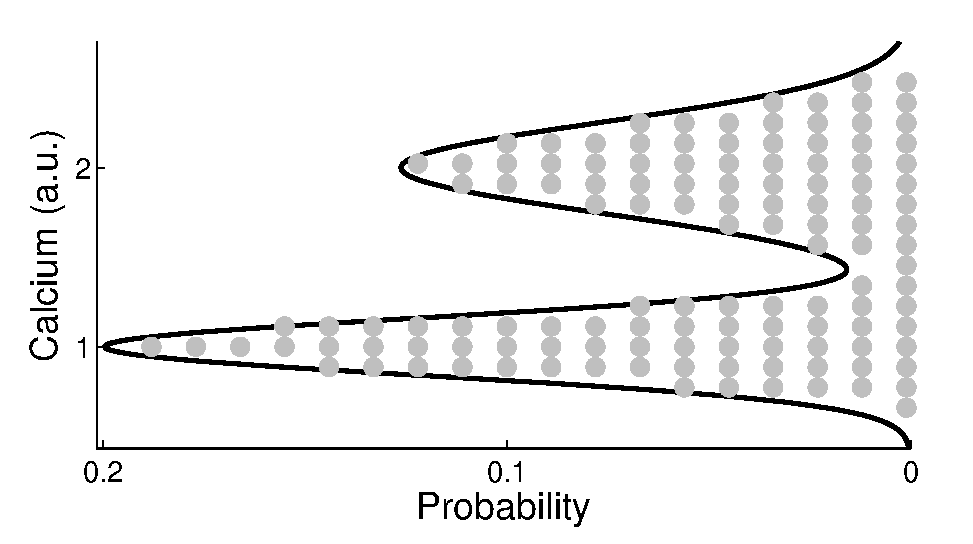
\includegraphics[width=1.0\linewidth]{PFapprox}
\caption[SMC]{Sequential Monte Carlo.  \textbf{(A)} A set of particles (gray dots) comprise a discrete approximation to the continuous mixture of Gaussians distribution (black line). \textbf{(B)} Approximating the $2^{v-s}$-component mixture with a $v-s+1$-component mixture.  The true conditional distribution (black line) is a mixture, with $2^{v-s}$ means (black $+$).  We approximate this mixture (gray line) with only $v-s+1$-components (each mean indicated by a gray $\times$).}
\label{fig:pf}
\end{figure}

%\begin{subequations} \label{eq:MPF0}
%\begin{align} \label{eq:MPF1}
%w_t^{(i)} &= \frac{1}{Z} \p[O_t | \ve{H}_t^{(i)}] \p[\ve{H}_t^{(i)} | O_{0:t-1}] \\ \label{eq:MPF2}
%\p [\ve{H}_t^{(i)} | O_{0:t-1}] = \sum_{j=1}^N \p[\ve{H}_t^{(i)} | \ve{H}_{t-1}^{(j)}] w_{t-1}^{(j)}
%\end{align}
%\end{subequations}

%\begin{multline}
\begin{align}\label{eq:MPF}
w_t^{(i)} = \frac{1}{Z} \p[O_t | \ve{H}_t^{(i)}] %\times \\
\sum_{j=1}^N \p[\ve{H}_t^{(i)} | \ve{H}_{t-1}^{(j)}] w_{t-1}^{(j)}
\end{align} %\end{multline}

Because the sum in \eqref{eq:MPF} requires computing the transition distribution for each pair of particles, one typically approximates \eqref{eq:MPF} with

%\begin{multline}
\begin{align}\label{eq:SIS0}
w_t^{(i)} = \frac{1}{Z} \p[O_t | \ve{H}_t^{(i)}] %\times \\
\p[\ve{H}_t^{(i)} | \ve{H}_{t-1}^{(i)}] w_{t-1}^{(i)}
\end{align}%\end{multline}

\noindent which is very accurate when the set of particles, $\ve{H}_{t-1}^{(1:N)}$, are close to one another (and therefore, have a similar weight).  To compute \eqref{eq:SIS0}, one must sample $\ve{H}_t^{(i)}$ from some distribution, which we will call the \emph{sampling distribution}\footnote{It is often referred to as the \emph{importance distribution} or \emph{proposal distribution}.}, $\q$.  An importance sampling argument informs us that upon approximating a distribution by sampling, one must normalize the likelihood by probability of having sampled that value (see \cite{Geweke89} for a discussion on using importance sampling for Bayesian filtering).  Therefore, one updates the particle weights using\footnote{Computing the weights using \eqref{eq:SIS} is typically referred to as Sequential Importance Sampling (SIS)\cite{LiuChen98}.  If one does not approximate \eqref{eq:MPF} with \eqref{eq:SIS0}, one if left with a result referred to as marginal particle filtering (MPF)\cite{KlaasDoucet05}.}

\begin{subequations} \label{eq:SIS}
\begin{align} \label{eq:SISa}
\widetilde{w}_t^{(i)} &= \frac{\p[O_t | \ve{H}_t^{(i)}]  \p[\ve{H}_t^{(i)} | \ve{H}_{t-1}^{(i)}] w_{t-1}^{(i)}}{\q} %, \qquad
\\ w_t^{(i)} &= \frac{\widetilde{w}_t^{(i)}}{\sum_j \widetilde{w}_t^{(j)}} \label{eq:SISb}
\end{align}
\end{subequations}

Therefore, to proceed with a SMC strategy, the only ``free parameter'' is the sampling distribution.  In the following section, we provide details for two options given the above model.  The first, called the \emph{prior sampler}, uses only the prior information to generate samples, meaning that it does not consider the observations as all.  The second, which we call the \emph{conditional sampler}, samples conditioned on the next observation.  While the prior sampler is conceptually simpler, it is far less efficient than the conditional sampler.

One final note on the use of SMC algorithms relates to the issue of \emph{resampling}. Because the particles are sampled according to the sampling distribution, some may be very unlikely, i.e., their weights are close to zero. When this happens, one can resample the particles by sampling (with replacement) particles according to their weights.  This tends to drop the unlikely particles and replicate the very likely ones. Of the several variants of the standard resampling approach have been proposed\cite{Rubin87, GordonSmith93, Whitley94, Kitagawa96, LiuChen98,  Fearnhead98, CarpenterFearnhead99}, we chose stratified resampling because of its efficiency and simplicity\cite{DoucMoulines05}.  Thus, to complete the SMC forward step, first initialize a set of $N$ particles to take some reasonable starting value, and assign each an equal weight.  Then, at each time step, (i) update the position (in hidden space) of each particle by sampling from the importance distribution; (ii) use \eqref{eq:SIS} to compute the weight of each particle; and (iii) resample if necessary. One iterates these three steps (together called Sequential Importance Sampling with Resampling (SIR)\cite{DoucetAndrieu00}) until arriving at $t=T$, at which time, the forward step is complete.

\subsubsection{SMC Backward Step}

Having completed the SMC forward step, the SMC backward step proceeds by substituting these weights into \eqref{eq:joint} to get the particle analog for the backwards recursion:

\begin{subequations} \label{eq:part_back}
\begin{align} \label{eq:part_joint}
&J^{(i,j)}_{t,t-1} = \p[\ve{H}_t^{(i)}, \ve{H}_{t-1}^{(j)} | \ve{O}] %\\&
=\p \big[\ve{H}^{(i)}_t | \ve{O}\big] \frac{
\p \big[\ve{H}^{(i)}_t | \ve{H}^{(j)}_{t-1} \big]
\p \big[\ve{H}^{(j)}_{t-1}  | O_{0:t-1}\big]}{\sum_j \p \big[\ve{H}^{(i)}_t | \ve{H}^{(j)}_{t-1} \big] \p \big[\ve{H}^{(j)}_{t-1}  | O_{0:t-1}\big]}
\\ \label{eq:part_marg} &M^{(j)}_{t-1} = \p[\ve{H}_{t-1}^{(j)} | \ve{O}]
= \sum_{i=1}^N J^{(i,j)}_{t,t-1}
\end{align}
\end{subequations}

\noindent where $M_t^{(i)}$ is the \emph{marginal} likelihood of particle $i$ taking value $\ve{H}_t^{(i)}$ at time $t$, conditioned on all the observations.  In other words, the set $\{M_t^{(i)}\}_{i=1}^N$ defines the discrete distribution of the hidden states at time $t$. Similarly, $J^{(i,j)}_{t,t-1}$ is the \emph{joint} likelihood of particle $i$ taking value $\ve{H}_t^{(i)}$ at time $t$ and particle $j$ taking value $\ve{H}_{t-1}^{(j)}$ at time $t-1$, conditioned on \emph{all} the observations. As such, the set $\{J^{(i,j)}_{t,t-1}\}_{i,j=1}^N$ is an $N\times N$ matrix defining the joint discrete distribution for particles taking values at neighboring time steps.  One therefore completes the backward step by initializing $M_T^{(j)}=1/N$ for all $j$, and then recursing \emph{backward} using \eqref{eq:part_back} to compute the marginal and joint conditional distributions until $t=0$.  At this point, the particle approximation of the E step is complete, and one may proceed to the M step. %and \eqref{eq:part_back} may be substituted into \eqref{eq:E_HMM} to obtain the particle approximation to $\Q$:
%
%\begin{multline}
%\widehat{Q}(\thetn,\theto) =
%\sum_{\substack{t\in\mathcal{T} \\ i,j \in [1,N]}} J_{t,t-1}^{(i,j)} \ln \p [\ve{H}_t^{(i)} |  \ve{H}_{t-1}^{(j)}] +
%\\ \sum_{\substack{t\in\mathcal{T}\\i\in[1,N]}} M_t^{(i)} \ln
%\p [O_t |  \ve{H}_t^{(i)}]
%\end{multline}
%
%\noindent Note that the integrals over hidden states have been replaced by sums over particles, corresponding to the particle approximation.

\subsubsection{SMC M Step}

Having the particle approximation to marginal and joint conditional distributions, they may be plugged into \eqref{eq:QT} and \eqref{eq:QO} to find the maximum likelihood estimate (MLE) of the transition distribution and observation distribution parameters

\begin{align} \label{eq:smcQT}
\ve{\theta}_T &= \max_{\ve{\theta}_T} \sum_{\substack{t \in\mathcal{T} \\ i,j \in[1, N]}} J^{(i,j)}_{t,t-1}  \ln \pT
[\ve{H}_t^{(i)} |  \ve{H}_{t-1}^{(j)}] \\ \label{eq:smcQO}
\ve{\theta}_O &= \max_{\ve{\theta}_O}  \sum_{\substack{t \in\mathcal{T}_o \\ i\in[1,N]}} M^{(i)}_t \ln \pO [O_t | \ve{H}_t^{(i)}]
\end{align}

\noindent completing one EM iteration.  As in the DT-SSM-EM algorithm, a SMC-EM algorithm proceeds by iterating (i) use the SMC forward-backward approach to find $\{J_{t,t-1}^{(i,j)}\}_{i,j=1}^N$ and $\{M_t^{(i)}\}_{i=1}^N$, (ii) and then plug them into \eqref{eq:smcQT} and \eqref{eq:smcQO} to maximize the parameters.  Upon convergence, one can perform the desired inference.  In particular, the probability that the neuron spiked at any time step is given by

\begin{align}
\widehat{p}_t = \sum_i M_t^{(i)} n_t^{(i)}
\end{align}

\noindent which follows from the fact that the mean of a Bernoulli distribution is simply its probability. Table \ref{tab:smc_em} provides pseudocode for implementing any arbitrary SMC-EM algorithm.

\subsection{SMC-EM for this Model}

Having these tools in our toolbox, we can now apply them to the above model. As mentioned above, when using a SMC-EM, having specified the model, the only remaining decision is what sampling distribution to use.  As such, we first develop a \emph{prior sampler} for this model, which is a relatively simple, but also relatively inefficient.  Then, we develop a \emph{conditional sampler}, which improves the prior sampler by sampling conditioned on the next observation. Finally, we show how to learn all the parameters of the model.



\subsubsection{Prior sampler}
\input{C:/D/Research/liam/SMC_EM_GLM/prior.tex}

\subsubsection{Conditional sampler}
%\documentclass{article}
%\usepackage{amsmath}
%\usepackage{a4wide}
%\providecommand{\ve}[1]{\boldsymbol{#1}}
%\newcommand{\thetn}{\ve{\theta}}
%\newcommand{\p}{P_{\thetn}}
%\title{k-mixture Conditional Sampler}
%\begin{document}
%\maketitle

More efficient sampling can be achieved by using a sampling distribution that explicitly considers the observations.  In particular, one can sample conditioned on the \emph{next} observation.  Thus, if $u$ is the time of the previous observation, and $v$ is the time of the next observation, for all $s \in(u,v]$, one would like to define $\q$ as $\p[\ve{H}_s|\ve{H}_{s-1}^{(i)},O_v]$, which may be expanded:

\begin{multline} \label{eq:XO_opt}
%\begin{split}
\p[\ve{H}_s|\ve{H}_{s-1}^{(i)},O_v] = \p [\{\ve{h},n,C\}_s | \{\ve{h},n,C\}_{s-1}^{(i)}, F_v]
\\ = \frac{1}{Z} \p \big[ \ve{h}_s | \ve{h}^{(i)}_{s-1}, n_{s-1}^{(i)} \big] \p \big[ n_s | \ve{h}^{(i)}_{s} \big] \p \big[ C_s | C^{(i)}_{s-1}, n_s^{(i)} \big] \p \big[ F_v | C_s \big]
%\end{split}
\end{multline}

\noindent where the only difference between \eqref{eq:XO_opt} and \eqref{eq:NO_opt} is the presence of the future observation probability,  $\p[F_v | C_s]$.  Thus, this future observation probability must be computed for all $s \in(u,v]$.  The idea for computing this future observation probability is depicted in Figure \ref{fig:pf}\textbf{(B)}.  At time $v$ (the time of the next observation), we have a Gaussian distribution governing where the calcium may be, centered at the observation value (this follows from \eqref{eq:F_t}) (black line at $v$, $+$ marks the mean). 

At $v-1$, the neuron could either have spiked or not.  If the neuron did not spike, for the calcium to be where it is at time $v$, the calcium should do the inverse of decay (remember that the recursion goes backwards).  However, if the neuron did spike, the calcium should be $\beta$ \emph{below} its value at time $v$.  In either case, because the noise on the calcium transitions is Gaussian, the distribution maintains its Gaussianity, and slightly increases its variance.  Thus, at time $v-1$, the distribution of calcium is a \emph{mixture of Gaussians}.  At $v-1$, we have a \emph{2-component mixture}, one component for $n_{v-1}=1$ and one for $n_{v-1}=0$ (black line at $v-1$, $+$'s mark the means for the 2 components). The component coefficient (probability of being in that component), $a_{n,v-1}$ is the expected probability of spiking or not.

Recursing backward one more step yields a 4-component mixture, as each component in the mixture at $v-1$ could have gotten there either from the neuron spiking or not at time $v-2$ (black line and $+$'s at $v-2$).  The coefficient for each of the 4 components is proportional to the expected probability of having that particular \emph{sequence} of spikes, i.e., at $v-2$, we have 4 possible sequences: $(00)$, $(01)$, $(10)$, and $(11)$ corresponding to no spikes, only spiking at time $v-1$, only spiking at time $v-2$ and spiking at both $v-1$ and $v-2$, respectively.  This suggests that at time $v-s$, there will be a $2^{v-s}$-component mixture, where each component may be indexed by a binary number of length $v-s$. 

An interesting observation is that at $v-2$, two of the means seem to be completely overlapping.  In fact, those two components correspond to $(01)$ and $(10)$, i.e., the sequences with exactly one spike.  This follows from the fact that the calcium time constant is much larger than the step size, $\tau_c \gg dt$; therefore, the amount of decay (or rather, inverse decay) in a few time steps is essentially negligible.  One can therefore approximate the two components corresponding to a single spike at $v-2$ into one Gaussian.  More generally, at any time $v-s$, all the components resulting from the same number of spikes between $s$ and $v$ can be combined into a single component.  One must simply take care to modify the component weights, means, and variances appropriately.  Upon doing so, at time $s$, instead of a mixture with $2^{v-s}$ components, we are left with a mixture of $v-s+1$ components (i.e., one component per possible number of spikes until time $v$)

This approximation drastically reduces the computational load of using the conditional sampler.  For instance, imagine that the frame rate, $f$, is $10$ Hz and the step size, $dt$, is $2$ msec.  In that scenario, without the approximation, there would be up to $v-u=1/(f dt)=50$ time steps between observations, yielding a $2^{50}$ component mixture in the no-approximation situation, versus a $51$ component mixture when using our approximation!  As such, we use this approximation for $\p[F_v | C_s]$ when sampling.  

Having $\p[F_v | C_s]$ for all $s\in(u,v]$, one can now sample from each of the hidden states by marginalizing \eqref{eq:XO_opt} with respect to the other hidden states.  For example, to construct to spike sampling distribution, $q[n_s]$, integrate out $\ve{h}_s$ and $C_s$ from \eqref{eq:XO_opt}:

\begin{align}
q[n_s] &\sim \frac{1}{Z} \iint  \p \big[ n_s | \ve{h}_s \big] \p \big[ \ve{h}_s | \ve{h}^{(i)}_{s-1}, n_{s-1}^{(i)} \big] \p \big[ C_s | C^{(i)}_{s-1}, n_s \big] \p[F_v|C_s] d\ve{h}_s dC_s
\end{align}

\noindent for both $n_s=0$ and $n_s=1$. Then, sample $n_s$ from this new Bernoulli distribution, which explicitly considers the observations.  One proceeds similarly to construct $q[\ve{h}_s]$ and $q[C_s]$, and then samples from those as well.  Having these sampling distributions, one must then compute the weights of each particle using

\begin{align} \label{eq:cond_w}
\widetilde{w}_s^{(i)} &= \frac{\p\big[O_s | \ve{H}_s^{(i)}\big]
\p\big[\ve{H}_s^{(i)} | \ve{H}_{s-1}^{(i)}\big] w_{s-1}^{(i)}}{q\big[\ve{h}_s^{(i)}\big] q\big[n_s^{(i)}\big] q\big[C_s^{(i)}\big]}
\end{align}

\noindent Then, at observation times, one resamples if appropriate.  Appendix \ref{sec:cond_samp} provides the mathematical details of how to compute $\p[F_v | C_s]$ and the sampling distributions, and Table \ref{tab:back} provides pseudocode for implementing the conditional particle filter, which can act as the forward step in the SMC-EM algorithm.

%\end{document} 

\subsubsection{Learning the Parameters}
\input{C:/D/Research/liam/SMC_EM_GLM/m_step.tex}

%\end{document} 